%%%%%%%%%%%%%%%%%%%%%%%%%%%%%%%%%%%%%%%%%%%%%%%%%%%%%%%%%%%%%%%%%%%%%%%%%%%%%%%%
%2345678901234567890123456789012345678901234567890123456789012345678901234567890
%        1         2         3         4         5         6         7         8

\documentclass[letterpaper, 10 pt, conference]{ieeeconf}  % Comment this line out
                                                          % if you need a4paper
%\documentclass[a4paper, 10pt, conference]{ieeeconf}      % Use this line for a4
                                                          % paper

\IEEEoverridecommandlockouts                              % This command is only
                                                          % needed if you want to
                                                          % use the \thanks command
\overrideIEEEmargins
% See the \addtolength command later in the file to balance the column lengths
% on the last page of the document

\usepackage{graphicx}
\usepackage{caption}
\captionsetup[table]{position=bottom}
% Use the postscript times font!
\usepackage{mathptmx}
\usepackage[per-mode=symbol]{siunitx}
\usepackage{bm}
%\usepackage{amsmath}
\usepackage{booktabs}
%\renewcommand\table{Table}

\usepackage{lipsum}

% The following packages can be found on http:\\www.ctan.org
%\usepackage{graphics} % for pdf, bitmapped graphics files
%\usepackage{epsfig} % for postscript graphics files
%\usepackage{mathptmx} % assumes new font selection scheme installed
%\usepackage{times} % assumes new font selection scheme installed
%\usepackage{amsmath} % assumes amsmath package installed
%\usepackage{amssymb}  % assumes amsmath package installed

\title{\LARGE \bf
Parallelizing Logistic Regression for Biological Experimental Design
}

%\author{ \parbox{3 in}{\centering Huibert Kwakernaak*
%         \thanks{*Use the $\backslash$thanks command to put information here}\\
%         Faculty of Electrical Engineering, Mathematics and Computer Science\\
%         University of Twente\\
%         7500 AE Enschede, The Netherlands\\
%         {\tt\small h.kwakernaak@autsubmit.com}}
%         \hspace*{ 0.5 in}
%         \parbox{3 in}{ \centering Pradeep Misra**
%         \thanks{**The footnote marks may be inserted manually}\\
%        Department of Electrical Engineering \\
%         Wright State University\\
%         Dayton, OH 45435, USA\\
%         {\tt\small pmisra@cs.wright.edu}}
%}

\author{Wansang Lim$$ and Valerie Angulo$$% <-this % stops a space
%\thanks{*This work was not supported by any organization}% <-this % stops a space
%\thanks{$^{1}$H. Kwakernaak is with Faculty of Electrical Engineering, Mathematics and Computer Science,
%        University of Twente, 7500 AE Enschede, The Netherlands
%        {\tt\small h.kwakernaak at papercept.net}}%
%\thanks{$^{2}$P. Misra is with the Department of Electrical Engineering, Wright State University,
%        Dayton, OH 45435, USA
%        {\tt\small p.misra at ieee.org}}%
}


\begin{document}



\maketitle
\thispagestyle{empty}
\pagestyle{empty}


%%%%%%%%%%%%%%%%%%%%%%%%%%%%%%%%%%%%%%%%%%%%%%%%%%%%%%%%%%%%%%%%%%%%%%%%%%%%%%%%
\begin{abstract} 
Logistic regression is a statistical analysis tool used as a predictive analytic in a variety of disciplines. In this paper, we focus on parallelizing logistic regression analysis as a predictive analytic for biological experimental design. Parallelizing logistic regression would improve computation time and decrease memory latency when analyzing large data sets, allowing for more data to be processed faster. In this paper, we compare a sequential implementation of a logistic regression model with a CUDA implementation, looking at the relationship between dataset sizes and time taken to process the data. Our findings point to performance improvements in computation time and greater data size processing for the CUDA version of logistic regression.

\end{abstract}


%%%%%%%%%%%%%%%%%%%%%%%%%%%%%%%%%%%%%%%%%%%%%%%%%%%%%%%%%%%%%%%%%%%%%%%%%%%%%%%%
\section{INTRODUCTION}

Logistic Regression is used as a predictive analytic in many disciplines ranging from biology and conservation to business. It models a binary dependent and one or more binary or nonbinary independent variables. This is useful in cases of observing phenomena that may occur due to a specific event. The purpose of logistic regression is to predict the occurrence of phenomena based on independent conditions. The binary dependent variable is either 0 or 1 and indicates the presence or absence of a certain condition, such as alive/dead or win/lose, that may be related to the independent conditions. In this paper, we are primarily concerned with the applications of logistic regression analysis for predictive analytics in biology.

Currently, there is an abundance of large datasets that are open sourced and easily accessible to the public. This is especially beneficial for scientific research. However, processing large data sets is time consuming and resource intensive for CPU in terms of memory and computation time. Sequential implementations of logistic regression require a lot of time to process smaller amounts of data and have a high memory latency \cite{c2}. Implementation of a parallelized logistic regression would allow for an increased amount of data to be processed in less time. In this paper, we compare a sequential implementation of logistic regression with a CUDA implementation, looking at the relationship between dataset sizes and time taken to process the data. Our findings point to improvements in computation time and ability to process larger data sets for the CUDA implementation of logistic regression.






\section{BACKGROUND}

Logistic regression describes the relationship between a binary dependent variable and one or many independent variables. The regression can be binomial, ordinal or multinomial and is based on linear regression in that it estimates a multiple linear regression function. This predictive analytic tool is useful in biology, data science and many other fields for predicting the odds of an event occuring based on independent factors. Following are the steps needed to implement a logistic regression.

\subsection{Linear Regression}
In order to do a logistic regression, we must first start with a linear regression.

$$Y = b_0 + b_1X_1 + b_2X_2 + b_nX_n$$

In this linear model, the $x_n$ are the predictors/independent variables and the $b_n$ are the parameters of the model or the coefficients of the independent variables, with $b_0$ being a constant term. The Y value is the outcome/dependent variable and can vary from negative to positive infinity for a linear regression \cite{c10} \cite{c1}. 

\subsection{Logistic Function}
The next step is to turn the linear regression into a sigmoid function, also known as a logistic function. 

$$Probability =  \frac{p(x)}{1-p(x)}   =   \frac{e^x}{1+e^x} 
= \frac{e^{(b_0 + b_1X_1 + ... + b_nX_n)}}{1+e^{(b_0 + b_1X_1 + ... + b_nX_n)}}$$

All of these forms are equivalent and are achieved by taking the exponential of both sides. P(x) is the probability of an outcome occurring and is divided by the probability that it will not occur (1-p(x)). This allows the range of values to be between 0 and 1, rather than negative infinity to positive infinity. However, this ratio provides a limited range of values, the odds of the probability must be taken to have a more continuous range of values \cite{c10}. 

\subsection{Logistic Regression} 
The core of logistic regression is to calculate the Y parameter, which is the log odds of an event occurring based on independent factors. The log odds is also known as the logit of the probability. To determine the logit, we must take the natural log of the logistic function. The purpose of this is to fit the logit of the probability of success with the predictors/x-values. We are then able to obtain a continuous predictor for the odds of an event happening \cite{c6}.

$$logit p(x) = ln[\frac{p(x)}{1-p(x)}]$$

After this step, the dependent variable turns into a logit variable. We are then able to estimate the probability of the occurrence of a particular event based on the independent variables. The logit serves as a link between the linear regression and logistic function.

$$ln[\frac{Y}{1-Y}] = b_0 + bX$$

Logistic regression seeks to find the equation that best predicts the value of Y for each value of X. The procedure to calculate Y involves matrix inversion after calculating the logit, which converts binary variables to continuous variables. This is where we have parallelized the logistic function.






\section{LITERATURE SURVEY}
We've looked at a variety of papers regarding parallelizing logistic regression, as well as the applications of parallelized and sequential logistic regressions. The following related works are presented because they either implement a biostatistic model of logistic regression or they compare sequential and parallel versions of logistic regression. 

\subsection{Biostatistic Logistic Regression Implementation}
The algorithm that we have coded sequential and parallel versions of is applicable to biology and environmental studies. In "Deforestation Modelling Using Logistic Regression and GIS", binary logistic regression is used to determine whether deforestation is present or not in an area based on slope as an independent variable. The use of logistic regression in this paper is what prompted us to parallelize logistic regression for biological applications. While a sequential version of the logistic regression is analyzed, there is no attempt to parallelize it. The data input is also far different than ours, where the focus is to use GIS with logistic regression. Bavaghar analyzes digital thematic-topographic maps with 63 different data layers such as forests, ranges and gardens. Our tests calculate B values from a matrix of randomly generated data, making data comparison with this work not possible \cite{c1}.

\subsection{Parallelizing Logistic Regression}
Other works have parallelized logistic regression for machine learning \cite{c2}. Liang, Choi et al. have looked at parallelized regressions in distributed platforms, parallel algorithms and sub-linear approximations. They worked with Hadoop and Spark, two distributed systems used in data science and analytics, to run sequential and parallel versions of code and compare platform/algorithm combinations with sub-linear algorithms specific to machine learning. This is clearly useful for machine learning but is not applicable to our purposes. Liang, Choi et al. focus on parallelizing machine learning algorithms that logistic regression utilizes, while we are looking to parallelize logistic regression as it applies to biology. They used five open datasets related to machine learning to make sure that they could accurately compare their methods whereas our data is randomly generated and doesn’t come from open source. Using open datasets are beneficial because the results allow for comparability with the performance of sequential machine learning algorithms that already exist. 

The work done by Peretti, Alessandro, and Francesco Amenta focuses on parallelizing logistic regression for the purposes of machine learning, bioinformatics and data analysis \cite{c3}. While it is primarily a machine learning approach and our work aims to be more generalized, the parallelization is reached by using CUDA parallel programming support, which we use in our experimental design as well. However, not much detail is gone into about how CUDA is implemented, only that different CUDA software versions are compared in determining the loss function for the machine learning logistic regression. Nevertheless, this work is useful in that it this approach is applicable to bioinformatics and data analysis. The dataset used is a real dataset containing anonymized patient information obtained from the Wisconsin Diagnostic Breast Cancer database. It contains 569 instances, with each instance corresponding to a patient. This work is beneficial because the results were acted upon, the predictor values were found to have a high level of accuracy. Given the estimated Y value obtained per patient, there was a better chance at predicting whether a patient had breast cancer or not.  


\subsection{Implementations Used or Referenced} 
In Evaluating Parallel Logistic Regression Models \cite{c2}, Liang, Choi et al. implement a binary logistic regression which we reference for the parallel algorithm approach, but we don't look at distributed platforms or sub-linear approximation. They analyze their experimental results in accuracy, efficiency, scalability, robustness and running time. We analyze our results in terms of performance time and data set size but use this work as a guide on how to analyze our results. 

From Bavaghar's work in Deforestation modeling using logistic regression and GIS \cite{c1}, we utilize logistic regression in the same context and proceed with the sequential code and parallelized code in a step-by-step approach as well. We break down our implementation into linear regression, logistic function and finally into logistic regression using our sequential and parallel code. Bavaghar uses $R^2$ chi square test to determine the fitness of the model, which is something we considered in our work but did not have enough time to do.

The main implementation that we reference are equations for a multiple regression model \cite{c9}. We use this to complete the final part of logistic regression, converting binary variables to continuous variables in order to relate logistic regression back to a linear model. We based our random data generation on Equation Set 1. 
$$Y = X \cdot B + e$$
The first column in our matrix contains Y values and the rest of the values are x values. We completed the majority of the logistic regression within our data generation, converting probability to the logit of the values in column 0, which is the dependent variable Y. Our programs for our sequential code and parallel code are based on Equation Set 2.
$$B = (X' \cdot X)^{-1} X' \cdot Y$$
This is where we transpose the matrix, compute matrix multiplication and inverse and get a parameter as output. From these parameters with are B value outputs, we can take new x values and obtain Y values that are the log odds of an event occurring for prediction. With open source data in the form of a matrix, we would be able to obtain meaningful Y values from our implementation of sequential and CUDA logistic regression.





\section{PROPOSED SOLUTION}
We aim to parallelize the logistic regression using CUDA for experimental designs in biology. There has been a lot of research on parallelizing logistic regression for machine learning techniques and algorithms, but nothing that we’ve seen that is general enough to cover parallelized logistic regression outside of machine learning purposes. The biostatistic research that we have come across uses sequential logistic regression with other new technologies but does not attempt to clarify parallelizing the logistic regression itself. There is no report about how much we gain by parallelizing logistic regression, and about optimum data size and structure to overcome communication overhead between the GPU and CPU, yet. Therefore, we propose to parallelize the logistic regression in order to improve predictive behavior in a number of fields. The purpose of this project is to show that logistic regression can be parallelized to analyze more data in less time and find the optimum condition for data size and structure.






\section{EXPERIMENTAL SETUP}

\subsection{Methods}
We decided to use a matrix of random values for our input data, where the user chooses the number of rows and columns. To make sure our generated data set is valid, we follow the assumptions of data used for logistic regression applications. This involves having a binary dependent variable, not having outliers present in the data or strong correlations between independent data sets, and making sure no x values are below -3.29 or above 3.29 \cite{c8}.

Our random data is composed of values between -3 and 3. We perform a logistic regression on the first values of each row by taking the logit, $ln[\frac{Y}{1-Y}]$, of all values in the first column, which then represents our Y values for each individual. Our rows therefore represent individuals (such as students, mice, etc) with a dependent Y and row-1 number of independent x’s. The column numbers are the number of independent x variables per row. We imagine that the Y values in our matrix are dependent on the random x values within each row, for experimental purposes. Our calculated Y values are not binary, they are meant to represent a grouping of individuals rather than a sole individual with a binary value. The purpose for this is because Toxicologists use this method for logistic regression and we want our project to match biological and environmental research. Viewing the data matrix, it can be seen that each row is presented as 
$$ln[\frac{Y}{1-Y}] = b_0 + b_1X_1 + b_2X_2 + b_3X_3$$
where we have one less independent x variable to account for the initial $b_0$ constant value. 

With this data as an input, to complete the logistic regression and fit the logit with the x values, we have to perform a simple regression on our matrix. Because we have multiple rows representing multiple groupings, we've chosen to use a multiple regression model on our logistic regression data to complete the regression. This multiple regression model is also used in biology for multiple variables. We based our implementation off of Equation Set 2 for the multiple regression formula \cite{c9}. 

For our sequential and CUDA code, we transpose the input matrix, multiply it with itself and take the inverse of this result. We then multiply the new result with the original transposed matrix and multiply this with our Y values in the first column. After this regression, we obtain B values, which can then be paired with new X values to produce the Y that is the log odds of an event occurring. Our sequential code contains recursion in the methods that take the inverse of the matrix. Our CUDA code utilizes Gaussian elimination in order to avoid recursion on the GPU. 

\subsection{Machine Setup} 

We used servers through NYU CIMS to run our sequential and parallel logistic regression programs. For the sequential program we used the snappy3 server, which is for CPU and memory intensive processes. We used the cuda2 server to run our CUDA program. Before running the programs, we ran our random data generator file to generate the appropriately sized matrix to test. We compiled the random data program and ran it with input arguments of number of rows and columns desired. From here, we compiled and ran our sequential or CUDA program with the matching row and column inputs of the data file we had generated. We used the time flag to record the time taken to compute the logistic regression of our sequential and CUDA code, and we used nvprof to profile our CUDA code. 

\subsection{Problem Size} 
We tested various problem sizes for sequential and CUDA programs, with the dimensions of the data matrix being much larger for CUDA than for the sequential code.  Because of the large degree of difference between the row input and column input, we don't focus too much on the size of the matrix so much as the actual dimensions. The data sizes for the sequential code range from a matrix size of 16 by 2 up to a matrix size of 100,000 by 6, where the first number is rows and the second number is columns. The size of the data matrix for the CUDA code ranges from 20 by 5 and 10 by 10 to 200,000 by 10 and 100,000 by 20. For CUDA, we tested much larger row and column numbers as well as smaller numbers to try to relate it with our sequential test sizes. We also tested dimensions greater than these ranges for both programs, but these attempts had varying successes.




\section{RESULTS AND DISCUSSION}

To analyze our results, we used time to determine the sequential and CUDA program performances, as well as whether the programs were able to successfully produce correct B value outputs. The time results used to produce our figures and Table 1 are averages of five times collected per each row and column value, in order to obtain more accurate results.

\subsection{Sequential Results}
The results for our sequential code show a very small difference per change in row value (Table 1). However, there is an increase in time with each increment of the column number, which appears to increase exponentially (Fig 1)(Table 1). Beyond column 12, we were unable to obtain results because time took longer than 1 hour, even when we use crunchy3 and snappy3 machines for quicker sequential computing. This limited our ability to properly compare our sequential results with our CUDA results. Differences in CUDA for column values as small as 2-12 did not provide us much insight.

Fig 1 shows that the difference between row number is very small, but the difference between column numbers with a constant row number begin to vary largely past column 8 (Table 1). We tested much greater row values (10,000, 50,000 and 100,000) to see if this made a difference between rows and it made a proportional difference. For example, the values (column = 6, row = 10,000) and (column = 6, row = 100,000) increase by a factor of 10 in row value and in time (Table 1). Through our results, we have seen that time increments $t^3$ past column 8 as the x variables (column  number) increase. We believe this is due to the recursion present in the sequential code, particularly in calculating the matrix inverse. In our sequential code, one of our recursive calls is "D += sign * A[index(0,f,N)] * determinant(temp, n - 1)". The parameter (n-1) is actually $(n-1)^2$ and is in a for loop, making it $n^3$, which matches the time it takes past column 8. Calculating the inverse of the matrix depends on our column number and not on row number, which is why column number makes such a large difference for increasing column numbers as opposed to row numbers. 

The NANs present in Table 1 are segmentation fault errors we received while attempting to obtain results for column numbers with row values of 10,000, 50,000 and 100,000.

\subsection{CUDA Results}

We checked if exponential performance difference depends on column number for our parallel code, as it does with our sequential code and found that the CUDA performance does not depend on column number up to 100 (Fig 2). So we focused on the number of rows for our CUDA code. Fig 2 shows that the column number of CUDA code up to 100 has no effect on performance. For our purposes, the number of independent variables, or column number in our project, is less than around 20 in papers for biology and environmental modeling. Because of this, we checked the effect of sample numbers while the column number is limited to 20. In both column number 10 and 20, the performance of CUDA code is unstable up to 1000 and 2000. After that, the performance is almost proportional to sample or row numbers (Fig 3 and Fig 4).

The nvprof for row number 1,000, 10,000, 100,000 and 200,000 is checked with column number 10 (Table 2). The time for CUDA matrix multiplication reduced proportionally with increase of row numbers from 1,000 to 200,000 and occupies over 85\%. Even in small number of rows such as 1,000, the time percentage for matrix multiplication is 99.89\%. This result indicates that our CUDA code is compute bound before the row number 200,000. 


\subsection{Comparing Both}

For the sequential code, at column 12, the time is around 400 seconds up to 1000 rows (Fig 1). We checked CUDA performance for the same condition. The time for CUDA code with a row of 1000 is dramatically reduced to 0.3 seconds, making it 1333 times faster than the sequential value.

For future work, we are planning to compare the algorithms for matrix inversion. For sequential code, we use adjoint and cofactor methods for matrix inversion. It uses recursion which is not easy to implement for CUDA code, and hinders usage of higher column values for sequential code. We used Gaussian elimination to get the matrix inversion for CUDA code. With this comparison, we can remove the difference in algorithm effects. Our row number limitation is about 100,000 ~ 20,000. We will try tiling for matrix multiplication to expand row numbers.  


%%%%%%%%%%%%%%%%%%%% SEQUENTIAL
   \begin{figure}[thpb]
      \centering
     % \framebox{\parbox{3in} {We suggest that you use a text box to insert a graphic (which is ideally a 300 dpi TIFF or EPS file, with all fonts embedded) because, in an document, this method is somewhat more stable than directly inserting a picture.
	 %}}
  		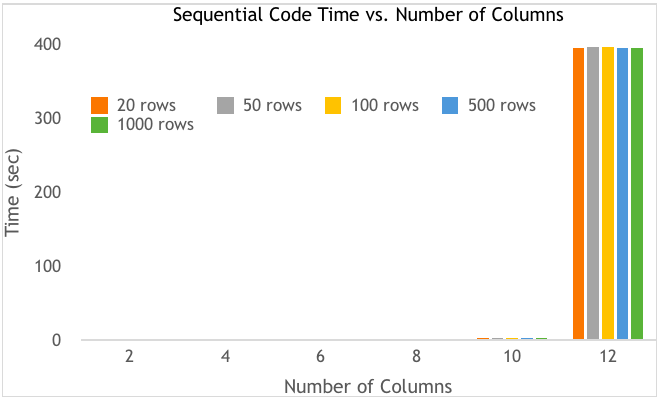
\includegraphics[width=\linewidth]{seqcode2.png}
  		\label{fig:seq1}
  		\caption{Sequential code performance for logistic regression with varying number of columns and rows. Each bar represents a different value for the row input, and all row values obtained are compared with column time values.}
  	%}
   \end{figure}
%%%%%%%%%%%%%%%%%%%% CUDA col
	\begin{figure}[thpb]
		\centering
		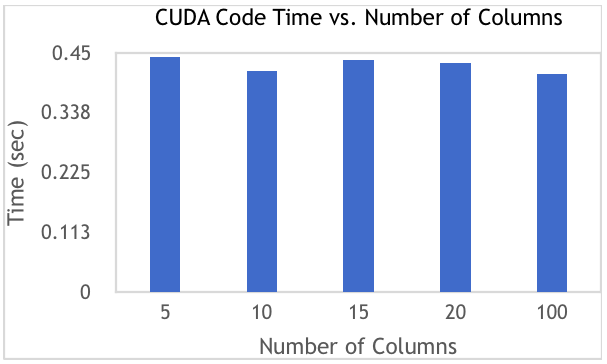
\includegraphics[width=\linewidth]{cudacolumns.png}
		\label{fig:cudacol}
		\caption{Performance difference of CUDA code between column number (5~20). The row number is set to 20 for all column numbers except for column = 100. The row number = 100 for column = 100.}
	\end{figure}
%%%%%%%%%%%%%%%%%%%% CUDA row=10
	\begin{figure}[thpb]
		\centering
		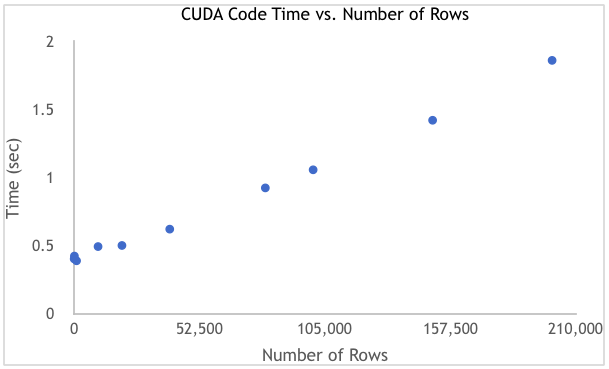
\includegraphics[width=\linewidth]{cudarow10.png}
		\label{fig:row10}
		\caption{Performance difference of CUDA code with a constant column value of 10.}
	\end{figure}
%%%%%%%%%%%%%%%%%%%% CUDA row=20
	\begin{figure}[thpb]
		\centering
		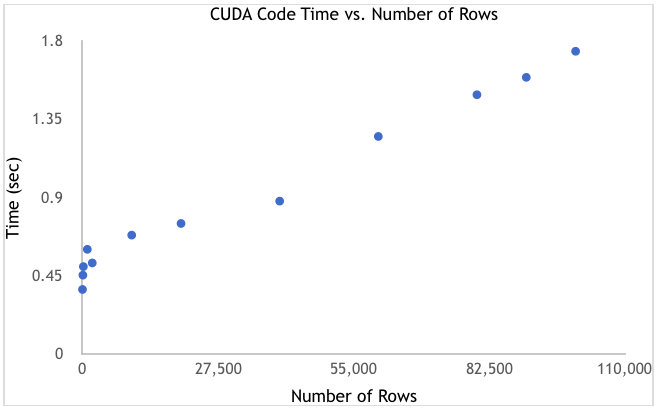
\includegraphics[width=\linewidth]{cudarow20.png}
		\label{fig:row20}
		\caption{Performance difference of CUDA code with a constant column value of 20.}
	\end{figure}	

\section{CONCLUSIONS}

The most important points of our project are listed below.

\begin{itemize}

\item The recursive nature of logistic regression in sequential code greatly limits the time it takes to compute increasing column numbers. 
\item CUDA code can handle large column numbers but there could be improvements with handling extremely large row numbers.
\item We would like to improve our CUDA code to make it more efficient in processing a larger sample size, such as row numbers of 1,000,000 or more.
\item We find that our CUDA code is much more effective at processing large column numbers quickly compared to our sequential code.
\item Our future work would include implementing Gaussian elimination in sequential code to make it more comparable to CUDA code.
\end{itemize}


%%%%%%%%%%%%%%%%%%%%%%%%%%%%%%%%%%%%%%%%%%%%%%%% ALL OF OUR FIGURES AND TABLES



%%%%%%%%%%%%%%%%%%%%%%%%%%%%%%%%%%%%%%%%%%

\begin{table*}[h]
\centering
%\caption{Sequential code time results per row and column value. Time is in seconds, these results were obtained through snappy3 CIMS machine.}
%\label{sequential}
\begin{center}
\begin{tabular}{|c|c|c|c|c|c|c|c|c|c|}
\hline
Col & Row = 16 & Row = 20 & Row = 50 & Row = 100 & Row = 500 & Row = 1000 & Row = 10000 & Row = 50000 & Row = 100000\\
\hline
2 & 0.0168 & 0.0104 & 0.0134 & 0.0116 & 0.0106 & 0.008 & 0.016 & 0.07 & 0.146 \\
\hline
4 & 0.016 & 0.01 & 0.0046 & 0.0112 & 0.0104 & 0.0082 & 0.025 & 0.112 & 0.228 \\
\hline
6 & 0.0148 & 0.0112 & 0.0062 & 0.0134 & 0.081 & 0.0096 & 0.034 & 0.157 & 0.31 \\
\hline
8 & 0.031 & 0.035 & 0.0276 & 0.0364 & 0.1254 & 0.032 & 0.066 & NAN & NAN \\
\hline
10 & 2.5764 & 2.602 & 2.615 & 2.5568 & 2.8394 & 2.5564 & NAN & NAN & NAN \\
\hline
12 & 397.905 & 395.137 & 396.281 & 396.541 & 395.702 & 395.609 & NAN & NAN & NAN \\
\hline
\end{tabular}
\caption{Sequential code time results per row and column value. Time is in seconds, these results were obtained through snappy3 CIMS machine.}
\label{sequential}
\end{center}
\end{table*}
%%%%%%%%%%%%%%%%%%%%%%%%%%%%%%%%%%%%%%%%%%%%%%%%%

\begin{table*}[h]
\centering
\begin{center}
\begin{tabular}{|c|c|c|c|c|}
\hline
operation & Row = 1,000 & Row = 10,000 & Row = 100,000 & Row = 200,000 \\
\hline
matrix multiplication & 99.89 & 99.49 & 90.81 & 85.96 \\
\hline
CUDA memcpy DtoD & 0.04 & 0.33 & 5.32 & 8.42 \\
\hline
CUDA memcpy HtoD & 0.03 & 0.08 & 3.78 & 5.55 \\
\hline
\end{tabular}
\caption{Time(percentage) of Profiling result from nvprof. The column number is set to 10}
\label{cudaprof}
\end{center}
\end{table*}

%%%%%%%%%%%%%%%%%%%%%%%%%%%%%%%%%%%%%%%%%%%%%%%%%%%%%%%%%%%%%%%%%%%%%%%%%%%%%%%%%%%%%%%%%%%%%%%%%%%%%%

\addtolength{\textheight}{-12cm}   % This command serves to balance the column lengths
                                  % on the last page of the document manually. It shortens
                                  % the textheight of the last page by a suitable amount.
                                  % This command does not take effect until the next page
                                  % so it should come on the page before the last. Make
                                  % sure that you do not shorten the textheight too much.

%%%%%%%%%%%%%%%%%%%%%%%%%%%%%%%%%%%%%%%%%%%%%%%%%%%%%%%%%%%%%%%%%%%%%%%%%%%%%%%%%%%%%%%%%%%%%%%%%%%%%%
%\section*{APPENDIX}

%Appendixes should appear before the acknowledgment.

\section*{ACKNOWLEDGMENT}

Thank you Professor Zahran for an excellent semester and for all your help.

\begin{thebibliography}{99}

%%%%%Chicago citation style
\bibitem{c9} Anthony. VBA9 - Multiple Regression Model. Accessed November 02, 2018. http://www.anthony-vba.kefra.com/vba/vba9.htm.

\bibitem{c1} Bavaghar, M. Pir. "Deforestation Modelling Using Logistic Regression and GIS." Journal of Forest Science 61, no. No. 5 (2016): 193-99. 

\bibitem{c2} Peng, Haoruo, Ding Liang, and Cyrus Choi. "Evaluating Parallel Logistic Regression Models." 2013 IEEE International Conference on Big Data, 2013. 

\bibitem{c3} Peretti, Alessandro, and Francesco Amenta. "Breast Cancer Prediction by Logistic Regression with CUDA Parallel Programming Support." Breast Cancer: Current Research 01, no. 03 (2016).

\bibitem{c4} Salame, Camil Wadih, Joaquim Carlos Barbosa Queiroz, Gilberto De Miranda Rocha, Mario Miguel Amin, and Edson Paulino Da Rocha. "Use of Spatial Regression Models in the Analysis of Burnings and Deforestation Occurrences in Forest Region, Amazon, Brazil." Environmental Earth Sciences 75, no. 3 (2016). 

\bibitem{c10} Schoonjans, Frank. "Logistic Regression." MedCalc. November 09, 2018. Accessed December 05, 2018. https://www.medcalc.org/manual/logistic\_regression.php.

\bibitem{c5} Singh, Sameer, Jeremy Kubica, Scott Larsen, and Daria Sorokina. "Parallel Large Scale Feature Selection for Logistic Regression." Proceedings of the 2009 SIAM International Conference on Data Mining, 2009, 1172-183. 

\bibitem{c6} Sperandei, Sandro. "Understanding Logistic Regression Analysis." Biochemia Medica, 2014, 12-18.

\bibitem{c7} Van, Phu Nguyen, and Théophile Azomahou. "Nonlinearities and Heterogeneity in Environmental Quality: An Empirical Analysis of Deforestation." Journal of Development Economics 84, no. 1 (2007): 291-309. 

\bibitem{c8} "What Is Logistic Regression?" Statistics Solutions. Accessed December 05, 2018. https://www.statisticssolutions.com/what-is-logistic-regression/.

\end{thebibliography}




\end{document}
